\section{Experiments}\label{sec:results}
%\marco{In my opinion, this introduction should go.}
To successfully perform the NA-task, the LSTM should encode and store at least two types of information: (1) the grammatical number of the subject; and (2) syntactic structure of the main subject-verb dependency. The latter information is important for identifying the time period during which the network should store the subject number,  and when it should output it and update number information. This section describes the `neural circuit' encoding this information in the LSTM.

\subsection{Long-range number units}\label{subsec:ablation}
\begin{center}
\begin{table}[ht]
\centering
\begin{tabular}{|P{2.3cm}|P{0.4cm}||P{0.6cm}|P{0.6cm}|P{0.6cm}|}
\hline
\B NA task & \B C & \B \unit{2}{\textbf{126}} & \B \unit{2}{\textbf{338}} & \B Full \\
\hline
\B Linzen & \B - &  ? &  ? &  ? \\
\hline

% Singular conditions

Simple & S & - &  - &  100 \\

Adv & S & - &  - &  100 \\

2Adv & S & - &  - &  99.9 \\

CoAdv & S & - &  \textcolor{red}{82} &  98.7 \\

namePP & SS & - &  - &  99.3 \\

nounPP & SS & - &  - &  99.2 \\

nounPP & SP &  - &  \textcolor{red}{54.2} &  87.2 \\

nounPPAdv & SS &  - &  - & 99.5 \\

nounPPAdv & SP &  - &  \textcolor{red}{54.0} & 91.2 \\


\hline
% Plural conditions
Simple & P &  - &  - &  100 \\

Adv & P &  - &  - &  99.6 \\

2Adv & P & - &  - &  99.3 \\

CoAdv & P &  \textcolor{blue}{79.2} &  - &  99.3 \\

namePP & PS & \textcolor{blue}{39.9} &  - &  68.9 \\

nounPP & PS &  \textcolor{blue}{48.0} & - &  92.0 \\

nounPP & PP &  \textcolor{blue}{78.3} & - &  99.0 \\

nounPPAdv & PS & \textcolor{blue}{63.7} &  - &  99.2 \\

nounPPAdv & PP & - &  - &  99.8 \\

\hline
\end{tabular}
\caption{Ablation experiments results: Percentage accuracy in all NA-tasks. Full: non-ablated model, C: condition, S: singular, P: plural. For tasks with two nouns, SS: singular-singular, SP: singular-plural, PS: plural-singular, PP: plural-plural. Red: Singular subject, Blue: Plural subject. \textbf{Shouldn't the Full column also be colored?} \textbf{Explain what do the dashes in the table mean.} \label{tab:ablation-results}}
\end{table}
\end{center}

We first measured LSTM performance on Linzen's data-set and on the various NA-tasks of Table
\ref{tab:data-sets}. Following
\newcite{Linzen:etal:2016} and later work, we compute the likelihood
that the LSTM assigns to the main verb of each sentence given the
preceding context, and compare it to the likelihood it assigns to the
verb inflected with the wrong number presented in the same
context. Accuracy in a given condition is the proportion of sentences
in the condition where the model assigned a higher likelihood to the
correct form than to the wrong one.%, and it is denoted $ACC_{NA−task}$.

Network performance is reported in Table
\ref{tab:ablation-results} (right column -- `Full'). We highlight
several aspect of these results. \textbf{Discuss Linzen} First, some NA-tasks and conditions
are clearly more difficult than others. For example, performance on
the Simple (0-distance) NA-task is better than that on the Co-Adv
NA-task, which in turn is better than that of the nounPP
tasks. Second, as expected conditions with an incongruent interfering
noun before the verb (the mismatch-number conditions of namePP, nounPP and
nounPPAdv) reduce network performance. %
% $ACC_{nounPP-SP}>ACC_{nounPP-SS}$ and
% $ACC_{nounPP-PS}>ACC_{nounPP-PP}$.
Last, for long-range dependencies, reliably encoding singular subject
across an interfering noun is more difficult than a plural subject:
for both nounPP and nounPPAdv, PS is easier than SP. A possible
explanation is that in English the plural form is almost always more
frequent than the singular one, as the latter only marks third person
singular, whereas the former is identical to the infinitive and other
forms. Thus, if the network reverts to unigram probabilities, it will
tend to prefer the plural. \textbf{We will have to say something about
  the Linzen results also re ablation.}

% $ACC_{nounPP-SP}<ACC_{nounPP-PS}$ and
% $ACC_{nounPPadv-SP}<ACC_{nounPPadv-PS}$ \yair{is it still the case in
%   the results?!}.
% Interestingly, this singular-plural asymmetry has
% been reported also in humans.

\subsubsection{Local vs. distributed code - an ablation study}
Number information may be stored in the network in either a local,
sparse, or a distributed way, depending on the fraction of active
units that carry it.  We hypothesized that if the network uses a local
or sparse coding, meaning that there's a small set of units that
encode number information, then ablating these units would lead to a
drastic decrease in performance in the NA-tasks.  To test this, we
ablated each unit of the network at a time, by fixing its activation
to 0, and tested on the tasks.

Two units were found to have exceptional effect on network performance
(Table \ref{tab:ablation-results}, \unit{2}{126} and \unit{2}{338}
columns). Ablating them reduced network performance by more than 10\%
across various conditions, and importantly, they were the only units
whose ablation consistently brought network performance to around
chance level in the more difficult incongruent conditions of the
namePP, nounPP and nounPPAdv tasks. A small subset of other units
also had an impact on network performance, but not as dramatically and
consistently as \unit{2}{126} and \unit{2}{338}
\footnote{\yair{report performance for these other
    units}}. The ablation effect depended on the
grammatical number of the subject: \unit{2}{126} significantly reduces
network performance only if the subject is plural and \unit{2}{338}
only if the subject is singular. In what follows, we will therefore
refer to these units as the `plural' and `singular' units, respectively,
or long-range number units when referring to both. Taken
together, these results suggest a highly local coding scheme of
grammatical number when processing long-range dependencies.

\subsubsection{Visualizing gate and cell-state dynamics}\label{subsec:gate-dynamics}
\begin{figure*}[ht]
%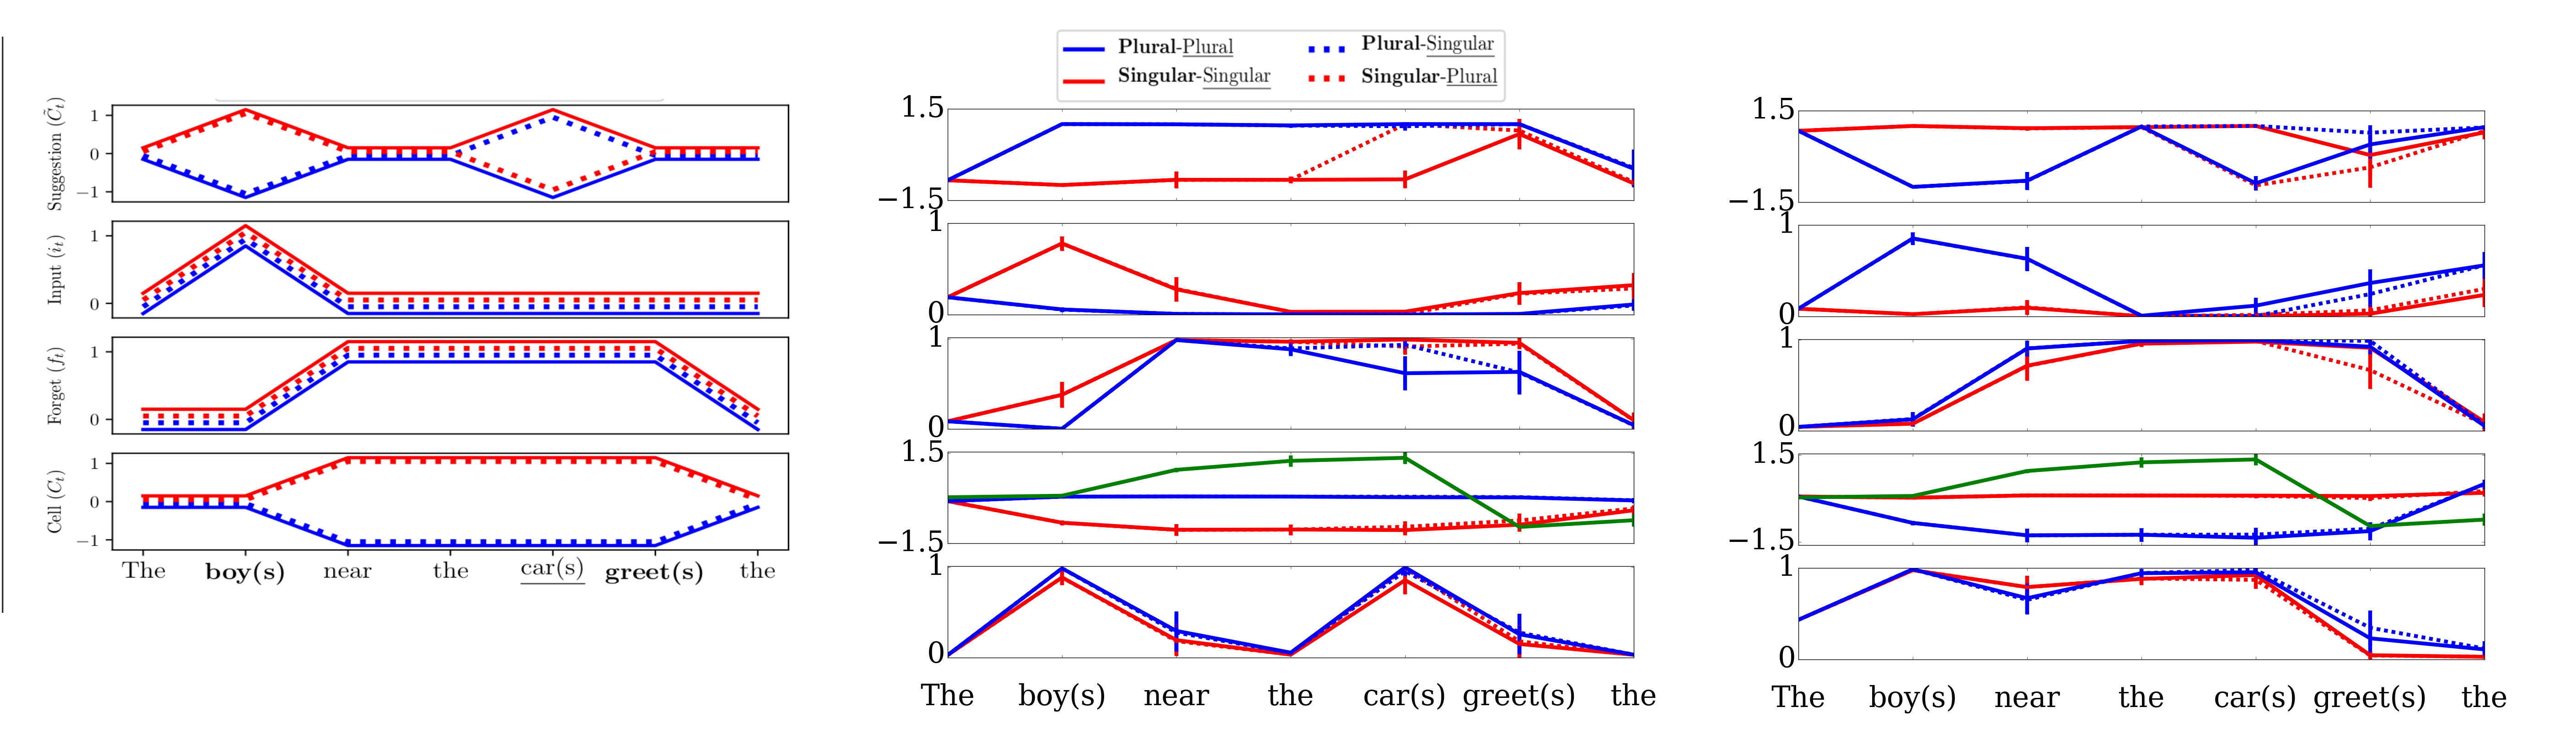
\includegraphics[width=\textwidth]{Figures/Figure2_cartoon_LR_units.png}
    \centering
    \begin{subfigure}{\textwidth}
            \centering
            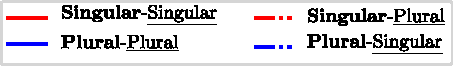
\includegraphics[width=0.3\linewidth]{Figures/legend.pdf}
    \end{subfigure}
    \bigskip
    \begin{subfigure}{0.32\textwidth}
            \centering
            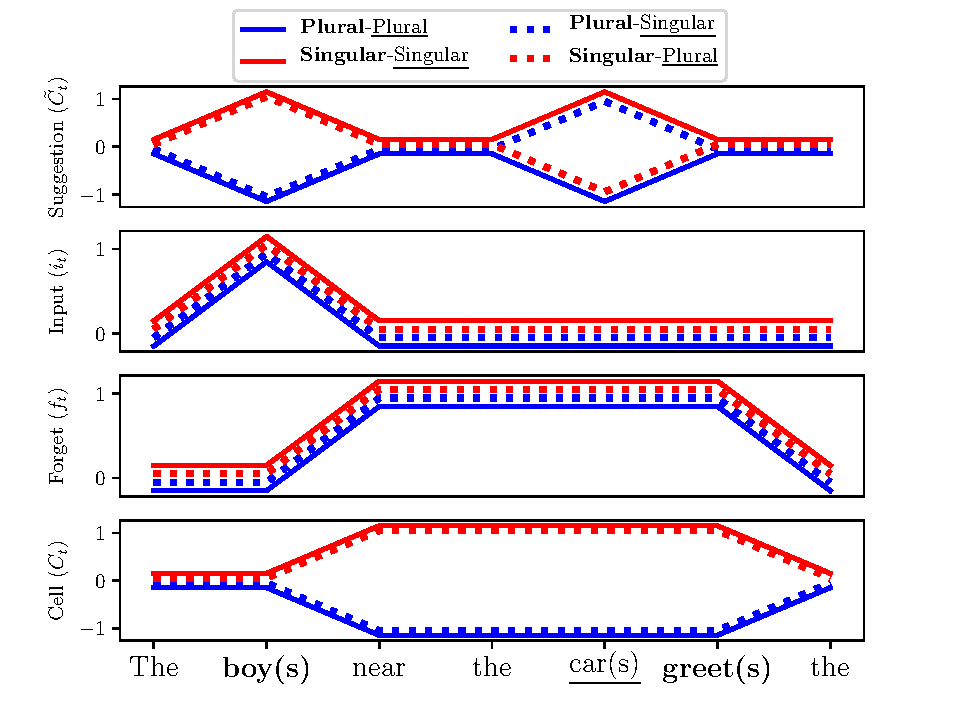
\includegraphics[width=\linewidth]{Figures/unit-timeseries-cartoon.pdf}
            \subcaption{Prediction (singular)}
    \label{fig:cartoon}
    \end{subfigure}
    \begin{subfigure}{0.32\textwidth}
            \centering
            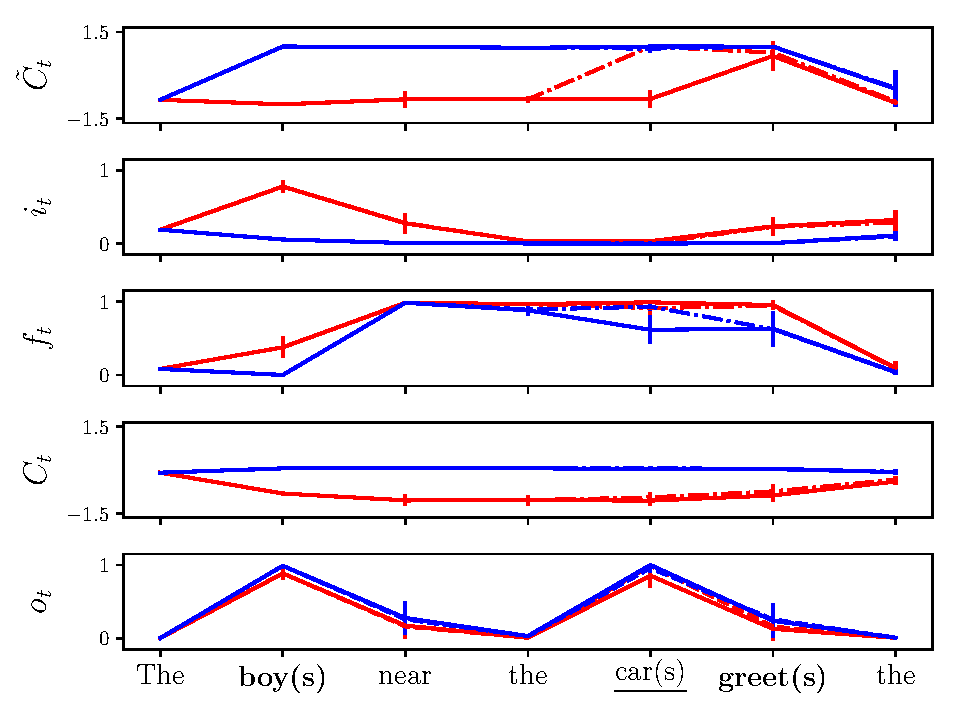
\includegraphics[width=\linewidth]{Figures/nounpp_987.pdf}
            \subcaption{Unit 998 (singular)}
    \label{fig:singular-unit}
    \end{subfigure}
    \begin{subfigure}{0.32\textwidth}
            \centering
            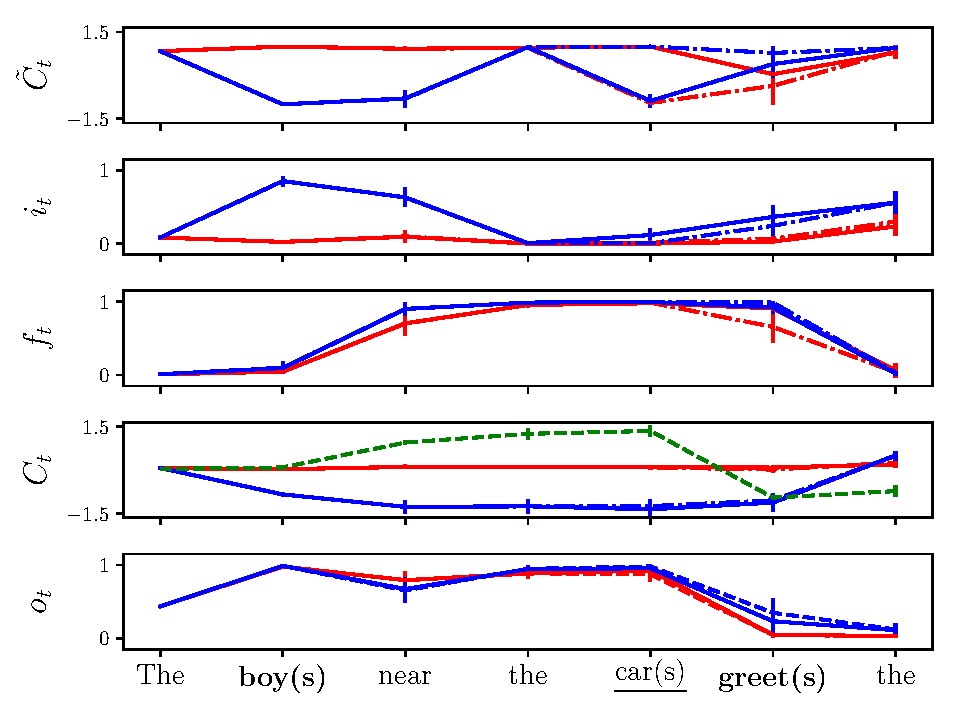
\includegraphics[width=\linewidth]{Figures/nounpp_775.pdf}
            \subcaption{Unit 776 (plural)}
    \label{fig:plural-unit}
    \end{subfigure}
\caption{Cell and gate activations during processing of a sentence with a prepositional phrase between subject and verb. Values in (b) and (c) are averaged across all condition sentences, with error bars showing standard deviations. \textbf{Change unit names to new layerwise notation.}}
\end{figure*}

To understand the functioning of the number units, we now look
into their gate and state dynamics during sentence processing. We
focus on the nounPP NA-task, which is the simplest NA-task including a
long-range dependency having an interfering noun, and both SP and PS
incongruent conditions.

Recall the standard LSTM memory update and output rules \cite{Hochreiter:Schmidhuber:1997}:

\begin{equation} \label{eq:update-rule}
     C_t = f_t\circ C_{t-1} + i_t\circ \widetilde{C}_t
\end{equation}

\begin{equation} \label{eq:output}
     h_t = o_t\circ \tanh(C_t)
\end{equation}

Consider now how a number unit may reliably encode and store subject
number across interfering nouns.  Figure\ref{fig:cartoon} exemplifies
this for a singular unit, showing the desired gate and cell
dynamics. The four conditions are represented with separated curves -
red for singular subject, blue for plural, and dashed lines for
incongruent conditions. Gate and cell activity at time points
unrelated to solving the NA-task are masked with white, as we do not
make precise predictions for them. The update rule of the LSTM cell
has two terms (Eq.~\ref{eq:update-rule}).\footnote{We abuse notation
  here, using the symbols normally denoting whole layers in
  (\ref{eq:update-rule}) and (\ref{eq:output}) to denote the elements of single
  cells.} In the first, $f_t \circ{} C_{t-1}$, the forget gate
controls whether to keep the previous cell content ($f_t=1$: perfect
remembering) or forget it ($f_t=0$: complete forgetting). In the
second term, $i_t\circ{} \tilde{C}_t$, the input gate controls whether
the information currently presented to the network, as encoded by
$\tilde{C}_t$, should be written onto the cell ($i_t=1$: full access)
or not ($i_t=0$). The singular unit can thus use these gates to
reliably store number information across long-range
dependencies. Specifically, the unit can: (1) encode subject number
via $\tilde{C}_{t_{subject}}$ with different values for singular and
plural; (2) open the input gate \textit{only} when a singular subject
is presented ($i_t=1$, red curves \textit{only}) and protect it from
interfering nouns ($i_t=0, t<t_{verb}$); (3) at the same time, clear
the cell from previously stored information ($f_{t_{subject}}=0$) and
then store subject number across the entire dependency
($f_t=1, t_{subject}<t<t_{verb}$); (4) finally, output subject number
at the right moment, when predicting verb form $o_{t_{verb}-1}=1$
(Eq.~\ref{eq:output}).

Figures \ref{fig:singular-unit} and \ref{fig:plural-unit} present the actual gate and cell dynamics of the singular and plural units. Both units follow the general solution for reliable number storage described above. Note that the plural unit `mirrors' the solution with respect to subject number (PP and PS vs.~SS and SP), which is in accordance with the results of the ablation experiments, that showed effect for only one value of subject number (table \ref{tab:ablation-results}). \textbf{I did not understand the previous sentence.} 

A single divergence between the solution depicted in Figure \ref{fig:cartoon} and the actual dynamics of the number units, is that input-gate activity is smaller, but not zero, at the time step immediately following the subject. One speculative explanation is that this might be useful to process compound nouns. In these cases, subject number information is stored with the second noun, whereas in the case of simple nouns there is no `risk' of encountering an interfering noun immediately after the subject, making the delay in closing the gate safe.

% \subsubsection{Predicting the verb form}\label{subsec:output-weight}

\begin{figure*}[t]
    \centering
    % GAT
    \begin{subfigure}{0.49\textwidth}
            \centering
            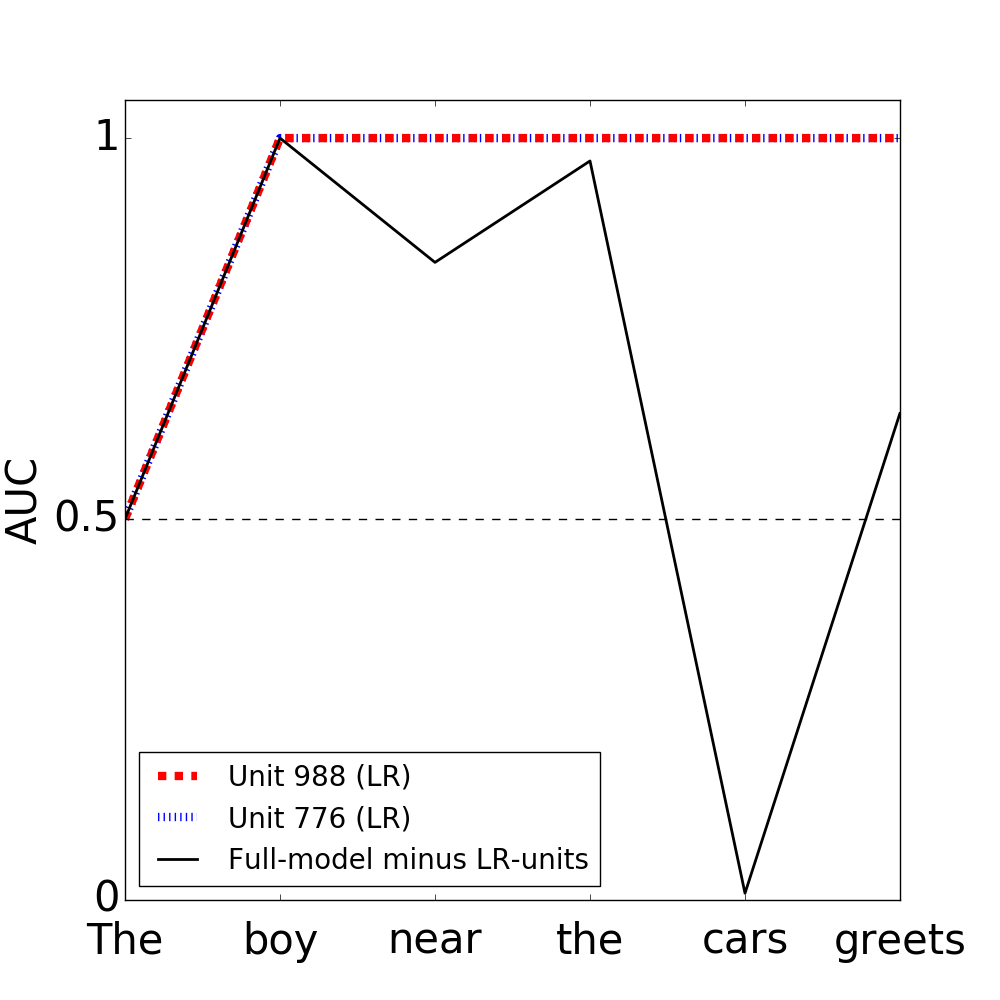
\includegraphics[height=5cm]{Figures/GAT1d_cell_nounpp_SR_LR_single_unit.png}
            \subcaption{Generalization across time.}
            \label{fig:GAT}
    \end{subfigure}
    \begin{subfigure}{0.49\textwidth}
            \centering
            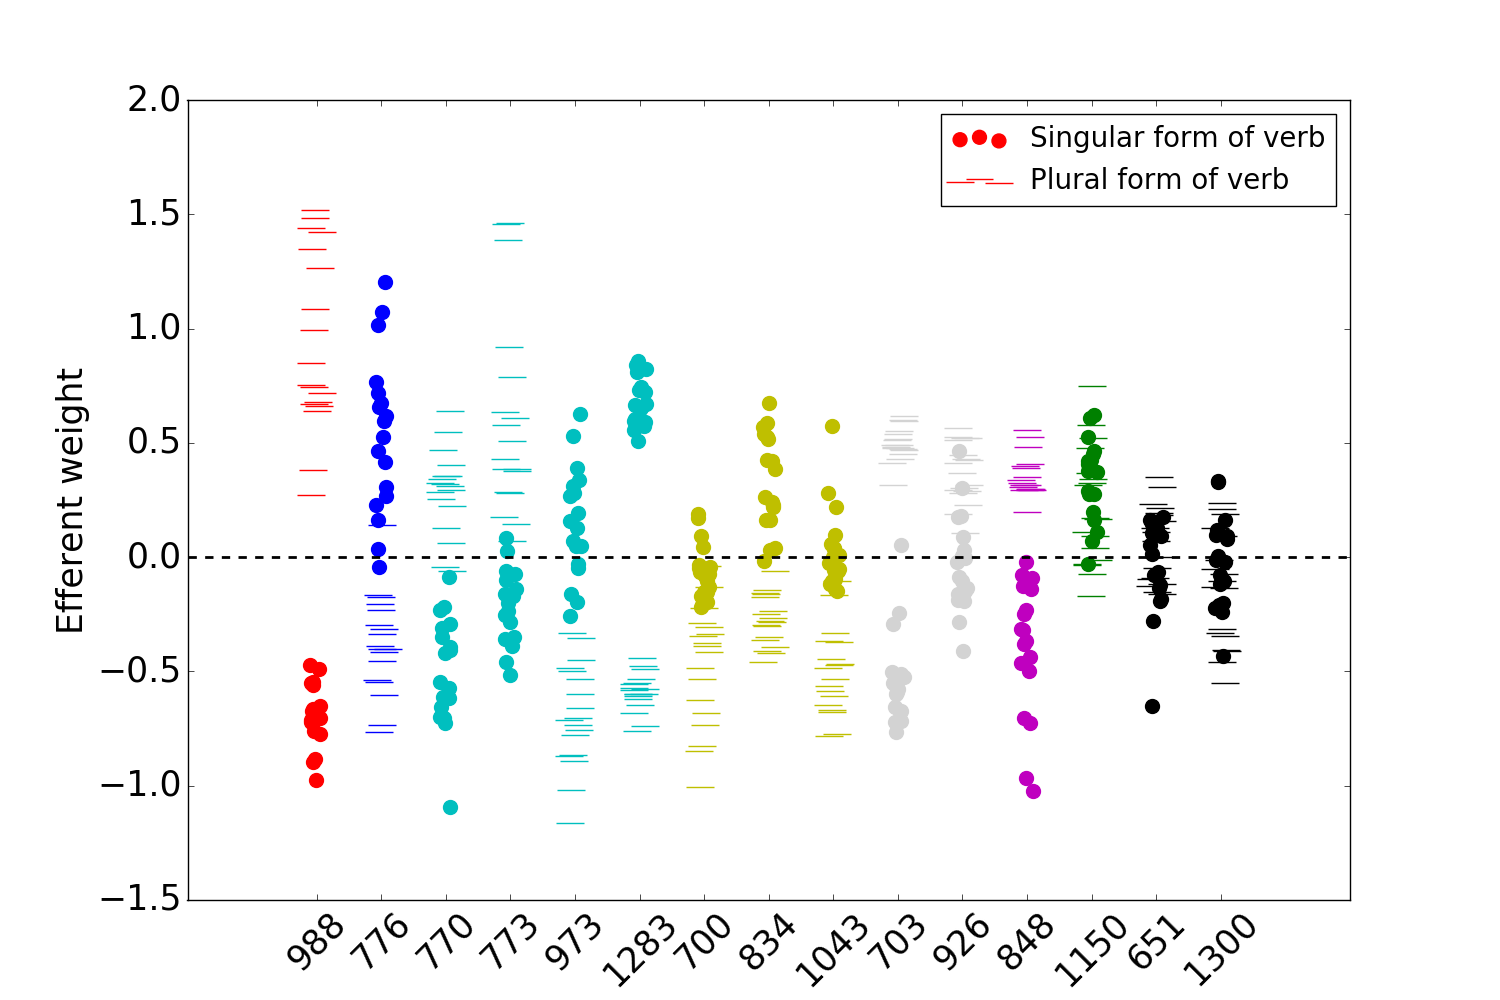
\includegraphics[height=5cm]{Figures/Figure5_output_weights.png}
            \subcaption{Efferent weights of number units.}
            \label{fig:output-weights}
    \end{subfigure}
    
\caption{(A) Generalization across time of network units. (B) Output weights of SR units, LR units, syntax unit, and two arbitrary units. \textbf{Something missing or out-of-date in the caption? Also, the second panel should go, right?}}
\end{figure*}

The singular and plural units have emerged at the second layer of the network. This seems appropriate if number information needs to be directly projected to the output layer for correct verb-form prediction. Moreover, number unit output should be projected differently to singular and plural verb forms in the output layer, only increasing activity in output units representing the suitable form. For example, for the singular unit, since singular subjects are encoded with a negative value ($C_{t_{verb}-1}<-1$ in figure \ref{fig:singular-unit}), the more negative its efferent weights to singular verb forms in the output layer, the higher the probabilities of these verb forms would be. Extracting the efferent weights of the number units to all verbs in our data-sets, we find that, indeed, the efferent weights to the singular and plural verb forms are segregated from each other \yair{singular unit: mean + std to plural, and mean+std to singular; plural unit: mean + std to plural, and mean+std to singular}, with weight signs that correspond to the negative encoding of subject number used by both singular and plural units.

\subsubsection{Short-range number information}
Performance on the easier NA-tasks (Simple, Adv, 2Adv) was not
impaired by single-unit ablations. This suggests that number may be
encoded also elsewhere in the network, perhaps via a more distributed
code. We tested whether subject number can be decoded from the whole
pattern of activities in the network (excluding the two number units)
and whether this decoding is stable across time \cite[see][for similar
observations and related methods]{Giulianelli:etal:2018}. We exepct
this distributed activity network to track number in a
small time window after the subject, but, unlike the proper number units,
to be affected by  incongruent intervening nouns.

We trained a linear model to predict the grammatical number of the
subject from network activity in response to the presentation of the
subject, and tested its prediction on test sets from all time points
\yair{cite King and Dehaene}, in incongruent conditions
only. \textbf{More details needed: across all NA-tasks? which test
  sets?} We used Area under of Curve (AUC) to evaluate model
performance. Figure \ref{fig:GAT} shows decoding across time of
subject number from cell activity of each number unit separately and
from cell activity of the entire network without these two units
(`Full model minus number units'). Results show that number
information can be efficiently decoded from other units in the
network, and that this information can be carried for several time
steps (relatively high AUC up to the second determiner). However, the
way in which these units encode number is sensitive to the last
encountered noun, with AUC decreasing to zero around the second noun
(`cars'), whereas test performance of the models trained on number
unit cell activity only is consistently high. This confirms our
hypothesis that number prediction is supported both by the number
units, and by distributed activation patterns of other units. The
latter mechanism, however, is not syntax-sensitive, and simply encodes
the number of the last noun encountered. \textbf{I'd remove the
  non-number units from the plot.} Qualitative inspection of cell and
gate dynamics of the units with the largest linear-model weghts
suggested they are considerably different from those of the
long-distance units, further suggesting that they encode number
information in a more opaque, distributed way. \textbf{There were
  several claims that there is a large number of SR units: if we have
  evidence for this (top weights in the linear mdoel?, it's worth
  mentioning.}

% This suggests a distinction between two types of units in the network: short-range (SR) vs. Long-Range (LR) number units. Only the latter type can carry subject-number information across LR dependencies with interfering nouns. Finally, we also evaluated decoding performance from cell activity of single units in the network that weren't found to decode number information ('non-number units'; Error-bars represent standard deviation across units). As expected, decoding performance is around chance level across the entire sentence. \yair{Do we want to explain how SR units were specifically identified (see commented-out part in this tex, from the previous version)? If not, we could take this part out also from the output-weight figure.}



%To quantify to what extent the efferent weights of each unit are segregated with respect to singular and plural verb forms, we used the statistical distance: $d^u_{W_P, W_S}=\frac{|\bar{W_S}-\bar{W_P}|}{\sigma_S+\sigma_P}$, where $W_S, W_P$ are the two sets of weights to singular and plural verb forms of unit $u$ with means $\bar{W_S}, \bar{W_P}$ and standard deviations $\sigma_S, \sigma_P$. 
%from units with both AUC values and $d^u_{W_P, W_S}$ within the top five percentile across all units. Figure \ref{fig:output-weights} presents the corresponding efferent-weight distributions from all number units, including the singular and plural units, and two arbitrary non-number units (units \unit{2}{1} and \unit{2}{650}). These results suggests that subject number is distributively encoded by the network for short-range dependencies without interfering nouns, and locally for LR dependencies with such interfering nouns.
